\chapter{Implementation}
	
	This chapter describes the implementation of the system in detail. First the
	electronics are described and followed by an explanation of the firmware.
	Finally, safety considerations and a brief discussion of the methods used is
	presented.
	
	
	\section{Electronics}
		
		% TODO: Some intro
		
		Two boards were produced, one which hosts the Mbed and the electronics
		needed to drive the heaters, motors and temperature sensors and another
		which provides an interface between the end-stops and stepper controller
		boards. The system as installed in the printer is shown in figure
		\ref{fig:electronicsPhoto} with the major components labelled.
		
		% TODO: Picture of up-to-date electronics
		\begin{figure}
			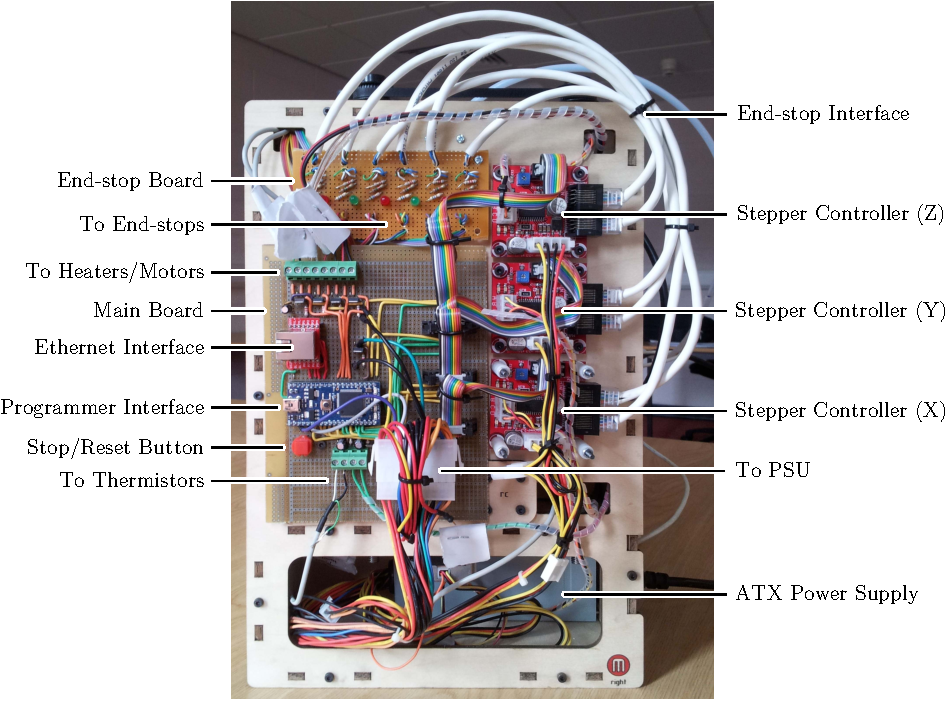
\includegraphics[width=1\textwidth]{diagrams/electronicsPhoto.pdf}
			\caption{Electronics installed with major connections labelled}
			\label{fig:electronicsPhoto}
		\end{figure}
		
		To keep the system simple to build using readily available tools, 0.1"
		spaced electronics were used throughout. These are easy to work with using
		only a standard soldering iron and basic tools. Components of this size can
		also be used in prototypes built on a solderless breadboard.
		
		The main board will host the Mbed, electronics for controlling the heaters,
		reading from the temperature sensors and connecting to the stepper
		controller boards. A second board is used for the end-stop electronics as
		these parts may be replaced separately from the main electronics and connect
		via the stepper controller boards.
		
		\subsection{Layout \& Board}
			
			A prototyping board designed for working with DIP (Dual In-line Package)
			components such as the Mbed was selected (Figure \ref{fig:dipBoard} B).
			Conventional strip board (\ref{fig:dipBoard} A) would require many
			connections to be cut between the two columns of pins of the device. The
			particular design chosen also includes a ready-made ground-plane.
			
			\begin{figure}
				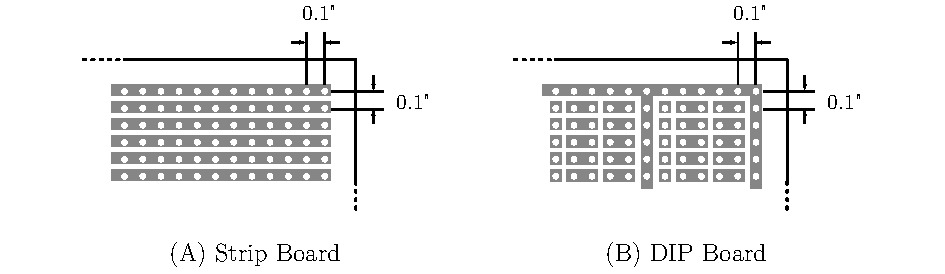
\includegraphics[width=1\textwidth]{diagrams/dipBoard.pdf}
				\caption{Types of prototyping board}
				\label{fig:dipBoard}
			\end{figure}
			
			\begin{figure}
				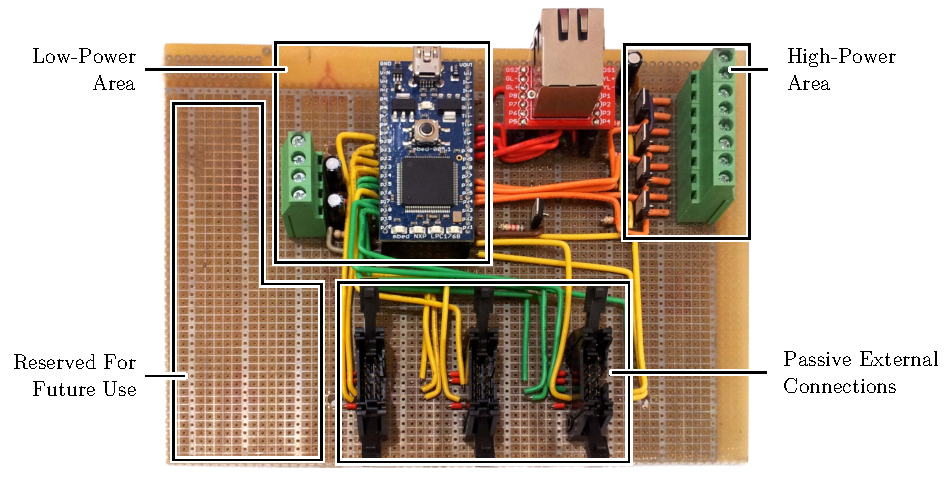
\includegraphics[width=1\textwidth]{diagrams/mainBoard.pdf}
				\caption{Top-level layout of main board (reset button and power
				         connections not shown)}
				\label{fig:mainBoard}
			\end{figure}
			
			The main board contains electronics for both low-power systems such as
			the Mbed and high-power systems such as the heater and motors and
			interference between these parts must be minimised. The high and lower
			power parts have been kept physically separate on the board (Figure
			\ref{fig:mainBoard}), each with their own power supply. The board also
			has a ground plane covering the whole board which also helps reduce
			noise\cite{pcb_design_notes}.
			
			A full circuit schematic and pin-out is given in Appendix
			\ref{sec:mainboardDiagrams}.
		
		\subsection{Heaters \& DC Motors}
			
			\label{sec:heatersAndMotors}
			
			% TODO: Part numbers, specs and fact check!
			
			The heaters and DC motors in the extruder and platform operate at a
			higher voltage and are considerably higher-current than the
			microcontroller can produce on its output pins. To control these a
			transistor is required.  An IRLU8729PbF MOSFET (Metal Oxide Field Effect
			Transistor) was selected as it can switch large loads up to 58A with
			very little on-resistance (reducing energy wastage through
			heat)\cite{MOSFET}.
			
			% TODO: Photo of MOSFET
			\begin{figure}
				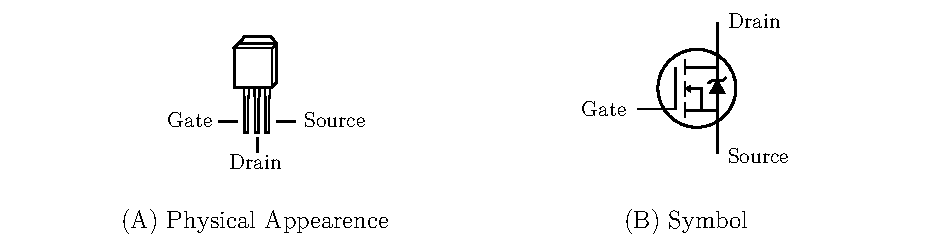
\includegraphics[width=1\textwidth]{diagrams/mosfetDiagram.pdf}
				\caption{Metal Oxide Semiconductor Field Effect Transistor (MOSFET)}
				\label{fig:mosfetDiagram}
			\end{figure}
			
			The MOSFET has three connections called the gate, drain and source
			(Figure \ref{fig:mosfetDiagram}). When the voltage between the gate and
			the source is 0V, no current flows from the drain to the source. As the
			voltage between the gate and drain are increased, the current allowed to
			flow increases rapidly when it passes a certain threshold (Figure
			\ref{fig:mosfetPerformance}). By connecting the gate to a pin on the
			Mbed and the source to ground, a large current from a device such as a
			heater or motor can be switched by connecting it through the drain to
			ground.
			
			\begin{figure}
				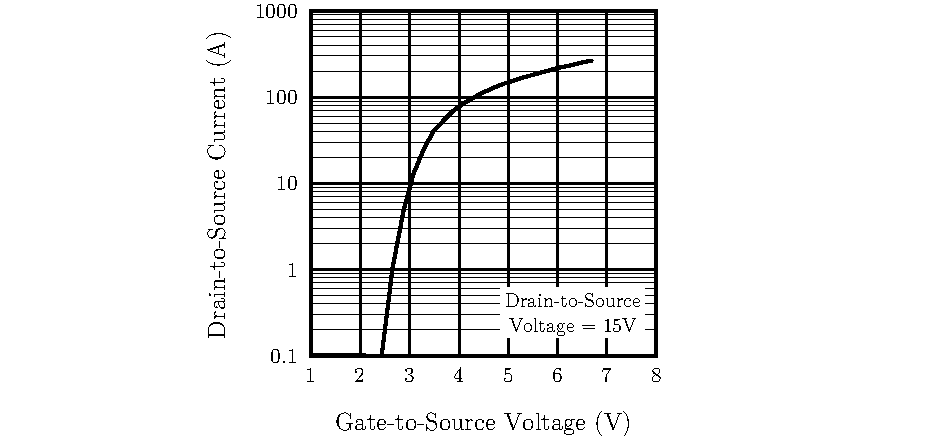
\includegraphics[width=1\textwidth]{diagrams/mosfetPerformance.pdf}
				\caption{IRLU8729PbF Typical Transfer Characteristics (reproduced from
				`Fig 3', \cite{MOSFET})}
				\label{fig:mosfetPerformance}
			\end{figure}
			
			The behaviour of a MOSFET when the gate is left floating (disconnected)
			is generally undefined and can damage the component. When the Mbed
			powers on its output pins default to a floating state which could cause
			a MOSFET to unexpectedly turn on or become damaged. To prevent this
			happening the gate is connected to ground via a pull-down resistor. When
			the output pin is floating the gate is pulled to 0V by the pull-down
			resistor. When the output of the pin is not floating, the gate is pulled
			to that voltage overriding the pull-down resistor. A high resistance
			value is used so that the Mbed can easily override the pull-down
			resistor.
			
			Figure \ref{fig:mosfetUsage} shows the circuit used to control the two
			heaters and two motors using a MOSFET and pull-down resistor.
			
			\begin{figure}
				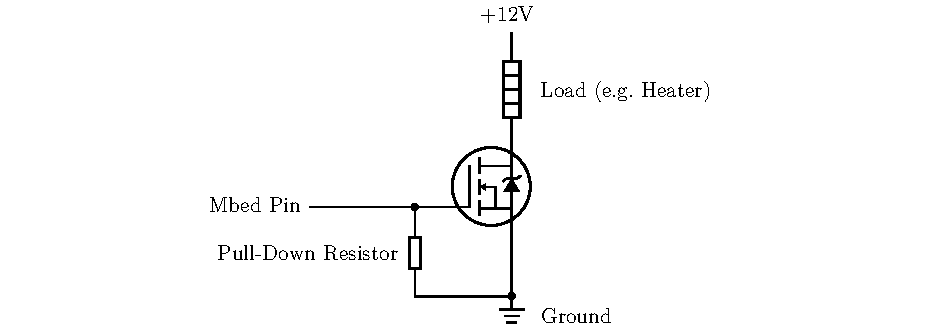
\includegraphics[width=1\textwidth]{diagrams/mosfetUsage.pdf}
				\caption{Example MOSFET circuit with pull-down resistor}
				\label{fig:mosfetUsage}
			\end{figure}
			
			When driving motors a `flyback diode' is usually used to prevent a
			voltage spike occurring when the power is removed from the motor. This
			voltage spike is caused by the magnetic field in the motor's coils
			collapsing. This is not included in the circuit as the MOSFETs used
			already contain an appropriate diode.
			
			It should be noted that this circuit does not allow the motors to be
			driven in both directions as this is not needed by the printer. If this
			was required, a more complex circuit (such as a H bridge) would be
			needed.
		
		\subsection{Thermistors}
			
			\label{sec:thermistor}
			
			To measure the temperature of the heaters, thermistors are used. The
			resistance of a thermistor changes non-linearly with temperature and is
			modelled using an equation derived from the Steinhart-Hart
			Equation\cite{Steinhart1968497}:
			\begin{equation}
				\frac{1}{T} = \frac{1}{T_0} + \frac{1}{\beta} \ln \left( \frac{R}{R_0} \right)
				\label{equ:steinhart}
			\end{equation}
			Where $T$ and $R$ are the current temperature and resistance of the
			thermistor, $T_0$ and $R_0$ are the temperature and resistance at a
			reference temperature and $\beta$ is a characteristic constant for the
			device available in the data-sheet.
			
			% TODO: Cite potential divider
			
			Using the Analog-to-Digital converter in the Mbed, voltages, but not
			resistances, can be read directly. A potential divider (Figure
			\ref{fig:potentialDiv}) is used to measure the resistance.
			\begin{figure}
				
\includegraphics[width=1\textwidth]{diagrams/potentialDiv.pdf}
				\caption{Potential divider}
				\label{fig:potentialDiv}
			\end{figure}
			A reference voltage $V_\textrm{ref}$ is placed across two resistors,
			$R_1$ and $R_2$, and the voltage between them at $V$ is measured. The
			relationship between these variables is
			\begin{equation}
				V = V_\textrm{ref} \frac{R_2}{R_1 + R_2}
			\end{equation}
			Thus, if the thermistor is placed as $R_2$, the resistance can be
			calculated using
			\begin{equation}
				R_2 = V_\textrm{ref} \frac{R_1}{V - V_\textrm{ref}}
				\label{equ:potdiv}
			\end{equation}
			
			% TODO: Resistor choice, specify thermistor
			
			The value of $R_1$ was chosen...
			
			Using (\ref{equ:steinhart}) and (\ref{equ:potdiv}) with a potential
			divider circuit will allow the temperature of the thermistor to be
			measured.
			
		
		\subsection{Stepper Motors}
			
			The stepper controllers chosen accept TTL signals and connect via a
			ten-pin insulation displacement connector (IDC). An IDC socket was
			placed on the board and the pins connected directly to the Mbed and
			ground plane as required. The pin-out for these connections is given in
			Appendix \ref{sec:stepperControllerPinout}.
			
			% TODO: IDC Picture
		
		\subsection{End-stops}
			
			Optical end-stops consist of a photo-interrupter containing an infra-red
			LED and a photo-transistor arranged across a gap (Figure
			\ref{fig:endstop}). Photons from the LED activate the photo-transistor
			allowing current to flow but when the gap is blocked, the transistor is
			switched off and no current flows.
			
			\begin{figure}
				
\includegraphics[width=1\textwidth]{diagrams/endstop.pdf}
				\caption{Photo-interrupter with a photo-transistor in a Darlington pair}
				\label{fig:endstop}
			\end{figure}
			
			Due to problems sourcing the interface boards for the end-stops, a
			circuit was built which is compatible with the stepper-controller
			interface for end-stops. $+5V$ and ground are provided and a TTL logic
			signal is expected by the interface. To ease debugging, an indicator LED
			is also provided which is lit when the end-stop is unobstructed.
			
			% XXX: Is it a pulldown?
			
			The LED in the photo-interrupter is driven via a current-limiting
			resistor and the signal output and indicator LED are connected through
			the photo-transistor. A pull-down resistor is used to pull the signal
			to ground when the photo-transistor is powered off.
			
			The circuitry is placed on a board with cables running to each end-stop
			(photo-interrupter) and to each of the CAT-5 sockets on the stepper
			controller boards. Strain-relief is included so that the connections are
			not damaged if the cables are caught in the machine. A circuit diagram
			is provided in Appendix \ref{sec:stepperControllerPinout}.
			
			% TODO: Picture of mounted endstop and board
			
			% XXX: Include resistor values and theory of operation?
			
			
		\subsection{Power}
			
			The printer uses an ATX power supply unit (PSU) commonly found in
			desktop computers. A 20-pin connector containing both power and various
			control signals for the power supply is used to power the main board
			(see table \ref{tab:atxConnectors}).
			
			\begin{table}[here]
				\centering
				\begin{tabular}{l l l}
					\toprule
					Signal & Colour & Notes\\
					\midrule
					Ground & Black  & \\
					+3.3V  & Orange & $\pm5\%$  Tolerance (Unused) \\
					+5V    & Red    & $\pm5\%$  Tolerance \\
					+12V   & Yellow & $\pm5\%$  Tolerance \\
					-12V   & Blue   & $\pm10\%$ Tolerance (Unused) \\
					\addlinespace
					Power Good  & Gray   & Signal asserted when all voltages are correct
					                       and stable \\
					+5V Standby & Purple & Power available at all times (Max 2A) \\
					+3.3V Sense & Brown  & Unused \\
					Power On    & Green  & Active-Low signal pulled up to +5V \\
					
					\bottomrule
				\end{tabular}
				
				\caption{20-pin ATX Connector Signals\cite{ATX}}
				\label{tab:atxConnectors}
			\end{table}
			
			The Mbed is connected to the 5V standby supply allowing it to remain
			booted and power on the system on demand. The maximum power consumption
			of the Mbed is 200mA \cite{mbed}, well within the ratings of the ATX
			specification. The Mbed's on-board regulator provides a regulated 3.3V
			supply used by the Mbed and the low-power electronics attached to it.
			The 3.3V supply from the PSU is not used because the regulator in the
			Mbed offers a cleaner supply.
			
			To allow the PSU to be turned on by the Mbed, the power on signal is
			attached to a GPIO pin.  Because the Mbed is a 3.3V logic device a
			MOSFET (Metal Oxide Semiconductor Field Effect Transistor) is used to
			pull the 5V Power On signal to ground (thus turning on the Power Supply)
			using the 3.3V signal from the Mbed.
		
		\subsection{Ethernet}
			
			Ethernet requires relatively complex circuitry to drive it. This is
			mostly provided on-board the Mbed but the pins on the mbed but a
			CAT-5 socket containing the magnetics required by Ethernet is needed.
			
			% TODO: Picture of magnetics?
	
	\section{Firmware}
		
		% TODO: Some intro
		
		\subsection{FreeRTOS on the Mbed}
			
			% TODO: Cite mbed compiler
			
			The Mbed is designed for use with a web-based IDE and compiler
			\cite{mbedcompiler}. This system is not appropriate for use in the project
			as the process of uploading code to be compiled is laborious and the
			compilation options restricted.
			
			The CodeSourcery G++ None-EABI toolchain includes a GCC ARM cross-compiler,
			linker and LibC compiled for various ARM based microcontrollers. It was
			selected over closed-source alternatives because it has a large community of
			users and produces reasonable code.
			
			% TODO: Cite CMSIS, LPC
			
			An unnoficial port of FreeRTOS for the Mbed is available which is built with
			the CodeSourcery toolchain. It provides a base FreeRTOS configuration with a
			demonstration \uIP{} based web server and other simple operating system
			demos along with a suitable Makefile. Also included are headders for the ARM
			Cortex Microcontroller Software Interface Standard (CMSIS) which define an
			interface for all ARM Cortex microcontrollers common features. Finally, the
			standard headders defining macros and pointers for all registers for the
			Mbed are included.
			
			Appendix \ref{sec:compilation} contains specific compilation instructions
			for the final system.
		
		\subsection{Temperature Control}
			
			To drive the two heaters an active-feedback loop is used where input from
			a thermistor (\S \ref{sec:thermistor}) is used to drive a heater via a
			MOSFET (\S \ref{sec:heatersAndMotors}). The following subsections describe
			how analog values are read by the Mbed and the theory and operation
			feedback loop that controls the heaters.
			
			\subsubsection{Analog Input}
				
				The Mbed includes a 12-bit successive-approximation analog-to-digital
				converter (ADC) for reading analog values\cite{LPC1768}. The ADC uses a
				digital-to-analog converter and a comparator to binary search for an
				approximation to the analog value (Figure \ref{fig:adc}). The input is
				held constant while the each bit in order of diminishing significance is
				determined. Once an appropriate number of iterations of the binary
				search have been carried out, the value in the register is returned
				\cite{maximadc}.
				
				\begin{figure}
					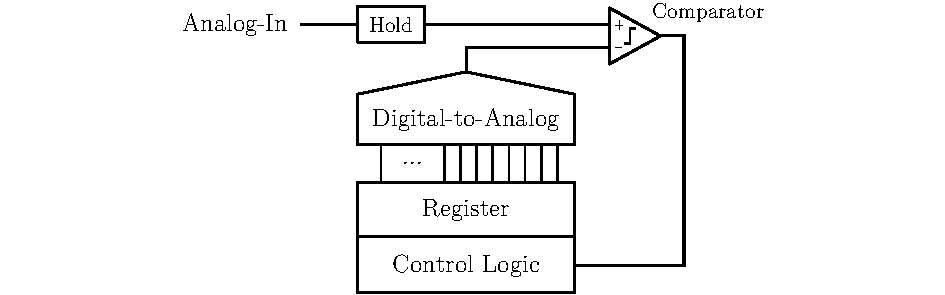
\includegraphics[width=1\textwidth]{diagrams/adc.pdf}
					\caption{Successive-approximation analog-to-digital converter}
					\label{fig:adc}
				\end{figure}
				
				The ADC sampling process takes at least $5\mu{}s$ or approximately 500
				CPU cycles \cite{LPC1768} therefore the CPU should carry out some other
				task while the ADC process takes place. Though an interrupt is provided
				when the ADC completes (and even a direct memory access (DMA) facility
				is provided), this was not used. The temperature sensors will be sampled
				at an extremely low rate (around 2Hz) and latency is not important as
				changes occur very slowly. Instead, a slow-poll is used where the task
				reading from the ADC is suspended for a time typically adequate for ADC
				operation. This system is extremely simple to implement and provides
				adequate read performance.
			
			\subsubsection{Control}
				
				A na\"{i}ve controller could simply turn on the heaters when the
				temperature was below some target temperature or `set point' and then
				off when it met or exceeded it. This controller would cause the
				temperature to overshoot and fall below the set point. Instead a
				proportional-integral-derivative (PID) controller is used which can
				control heaters taking into account such behaviours. These controllers
				are widely used and are often used when a process must be controlled
				which is not completely understood \cite{controleng}.
				
				\begin{figure}
					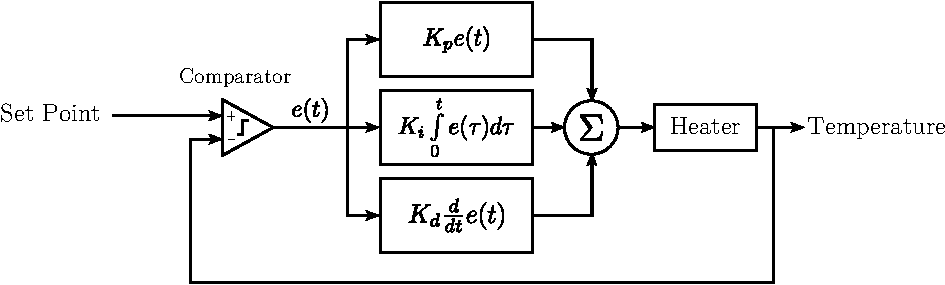
\includegraphics[width=1\textwidth]{diagrams/pid.pdf}
					\caption{PID heater controller schematic}
					\label{fig:pid}
				\end{figure}
				
				Figure \ref{fig:pid} shows a schematic of the PID controller used in the
				system. At time $t$ the comparator calculates the error $e(t)$ between
				the actual temperature and the set point. A value is calculated from
				this error using a factor proportional to the error, the error
				accumulated over time (integral) and the error's rate of change. These
				factors are weighted by the constants $K_p$, $K_i$ and $K_d$
				respectively and then used to control the heater. The three weights must
				be chosen manually to produce sensible behaviour.
				\S\ref{sec:pidtraning} discusses the process of selecting these values.
				
				The value calculated could be used with an analog output or
				PWM\footnote{Pulse width modulation (PWM) is a method of approximating
				analog outputs by rapidly switching a signal on and off with a varying
				duty-cycle. This is cheap to implement in hardware and also avoids
				problems with inefficiencies in MOSFETs when only partially driven.} to
				control the heater or a threshold value used to decide whether a heater
				is on or off (`bang-bang' control). Bang-bang control has been used
				because the previous electronics proved this to be adequate. Using PWM
				to control the heaters may also have resulted in unwanted
				electromagnetic noise.
				
				The PID control loop is executed in its own task at a rate of 2Hz where
				each temperature is read and the heater switched on or off as
				appropriate. Because of the slow rate of change this is an adequate
				response speed. Executing the loop more frequently would not be useful
				and, due to floating point calculations being carried out in software,
				would be costly.
		
		\subsection{Stepper Control}
			
			\subsubsection{Timers}
			
			\subsubsection{Timing}
		
		\subsection{G-Code Interpreter}
			
			\subsubsection{The G-Code Machine}
			
			\subsubsection{Instruction Selection}
			
			\subsubsection{Parsing}
		
		\subsection{System Control}
		
		\subsection{Network Interface}
			
			\subsubsection{G-Code}
			
				\subsubsection{TCP}
				
				\subsubsection{UDP}
			
			\subsubsection{Status}
	
	\section{Utilities}
		
		\subsection{G-Code Sender}
		
		\subsection{Status Monitoring}
	
	\section{Safety}
		
		\subsection{STOP Button}
		
		\subsection{Watchdog}
		
		\subsection{Power-on Behaviour}
	
	\section{Methodology}
		
		\subsection{Tools}
			
			\subsubsection{Git (Version Control)}
			
			\subsubsection{Wireshark (Network Protocol Analyser)}
		
		\subsection{Languages}
			
			\subsubsection{C}
			
			\subsubsection{Python}
		
		\subsection{Debugging}
